\documentclass{article}

% Packages
\usepackage[utf8]{inputenc}
\usepackage[T1]{fontenc}
\usepackage{lipsum} % For dummy text
\usepackage{physics} % For physics notation
\usepackage{amsmath} % For math
\usepackage{amssymb} % For math symbols 
\usepackage[margin=2cm]{geometry} % For smaller margins
\usepackage{gensymb} % For degree symbol
\usepackage{diagbox} % For table
\usepackage{slashbox} % For table
% \usepackage[margin=1in,headheight=57pt,headsep=0.1in]{geometry}
\usepackage{hyperref}
\usepackage{xcolor} % for colored text
\usepackage{graphicx} % For \includegraphics
\usepackage{float}    % For the [H] placement specifier

% Document information
\title{FYP Report}
\author{Lin Zhonglin}
\date{\today}

\begin{document}
\noindent

\maketitle
\tableofcontents

\section{Overview}
\begin{enumerate}
    \item Background: 
    \item Key part of my work: (depends on how far I go)
        \begin{enumerate}
            \item The optimised pulse for a particular state preparation
            \item how it differs from other pulse (Chiyuan's alternate pulse way)
            \item Go from model Hamiltonian to physical Hamiltonain, 
                    discuss the approximations' effect, 
                    compare fideilty
        \end{enumerate}
\end{enumerate}

TODO: 
\begin{enumerate}
    \item Go through the Hamiltonian derivation 
            $\rightarrow$ for comparison of fidelity later 
    \item does Qutip considers the cavity Hilbert space truncation discussed below? 
\end{enumerate}


Issues to be dealt with: 
\begin{enumerate}
    \item local minima / maxima in optimization algorithm
    \item Reinhold: 
        Optimizing a full unitary operation is sensible for qubits, or systems of a few qubits, but in the cavity manipulations to be performed in the following sections, this is not usually a sensible operation, since doing operations involving states at the border of the truncation (i.e. the maximum photon number state considered in the simulation), would typically require a larger truncation to simulate accurately (driving $\ket{n_{ph}}$) will almost always in part bring us partially to $\ket{n_{ph} + 1}$.
\end{enumerate}


%%%%%%%%%%%%%%%%%%%%%%%%%%%%%%%%%%%%%%%%%%%%%%%%%%%%%%%%%%%%%%%
\section{Background, theory and motivation}
%%%%%% 草稿 %%%%%%%%
content: 
introduce the idea of bosonic-modes-encoded qubits, give a simple example;
motivate Bosonic-modes-encoded qubits 
    -> that one physical device now can encode multiple qubits
    -> this also makes error correction more efficient -> easier to control multiple qubits

introduce cavity-transmon system 
motivate for cavity-DQD system

theory of cavity-DQD: 
original Hamiltonians -> rotation, approximaition, dispersive regime, etc... -> the Hamiltonian I used for pulse optimization

briefly bridge to and cover the overview of content of this report: 
1. basic theory on optimization, QuTip, GRAPE, CRAB, etc...
2. pulse optimization for state preparation
3. compare fidelity from approximate Hamiltonian with fidelity from original Hamiltonian 
4. possible future work: gate design, model noise
%%%%%% 草稿 %%%%%%%%

%%%%%%%%%%%%%%%%%%%%%%%%%%%%%%%

%%%%%%%%%%%%%%%%%%%%%%%%%%%%%%%%%%%%%%%%%%%%%%%%%%%%%%%%%%%%%%%
\subsection{Hamiltonian of system}

%%%%%%%%%%%%%%%%%%%%%%%%%%%%%%%
\subsubsection{Transmon-cavity system}

%%%%%%%%%%%%%%%%%%%%%%%%%%%%%%%
\subsubsection{DQD-cavity system}

\subsection{Optimal control}
We assume we have a quantum system, whose Hamiltonian can be written in the following form: 

\begin{equation}
    H(\vec{\epsilon}(t)) = H_0 + \sum_{k=1}^m \epsilon_k(t) H_k
\end{equation}
Goal: Find optimal control field $\vec{\epsilon}(t)$ that optimizes some function $f(\vec{\epsilon}(t)) = f(H(\vec{\epsilon}(t)))$. \\
\begin{enumerate}
    \item To optimize a large number of parameters, we need:
        \begin{enumerate}
            \item an efficient means of calculating the gradients of cost function w.r.t parameters
            \item sub-optial local minima are sufficiently unlikely or close to global minima
        \end{enumerate}
    \item Given methods to calculate cost function and gradients, we have two main classes of algorithm for performing optimization: 
        \begin{itemize}
            \item line-search methods: one alternates between picking a direction in parameter space, radiating from our current point, and subsequently performing a 1-d minimization protocol to find the minimum along this line. \\
                $\rightarrow$ basic gradient descent: choose direction as gradient at the point. \\
                $\rightarrow$ Newton method: choose direction using both gradient and Hessian matrix at the point. $\rightarrow$ quasi-Newton, L-BFGS
            \item trust-region methods
        \end{itemize}
    \item calcualte gradient of $f(\vec{\epsilon}(t))$ with respect to $\vec{\epsilon}(t)$
        \begin{enumerate}
            \item For an analytical function $f(\vec{\epsilon})$, gradient is given by $\nabla f(\vec{\epsilon}) = \sum_{i=1}^m \frac{\partial f(\vec{\epsilon})}{\partial \epsilon_i} \hat{\epsilon}_i$
            \item For discrete $\vec{\epsilon}$, gradient of $f(\vec{\epsilon})$ is given by the finite difference method.
            \item approximate the gradient: skipping here.
            \item When calculating / approximating gradient is too expensive, cosider optimization algorithm other than gradient descent.
        \end{enumerate}
    \item take a step (step size as a parameter) in the direction. \\
        step size too small: optimization takes long\\
        step size too large: may never reach true optima
    \item calcualte gradient again
    \item repeat until convergence
    \item issue of local minima / maxima: 
        \begin{itemize}
            \item Optimize for infidelity (1 - fidelity) instead of fidelity. 
                Because infidelity is lower bounded by 0. Terminate optimization when infidelity reaches 0 or close to 0. 
        \end{itemize}
\end{enumerate}

%%%%%%%%%%%%%%%%%%%%%%%%%%%%%%%
\subsubsection{Figure of merit, cost function}
state transfer case
single-state state transfer: 
\begin{align*}
    f(\vec{\epsilon}(t)) &= \mathcal{F}(\vec{\epsilon}(t)) \quad \text{state fidelity}\\
    &\equiv \abs{\bra{\psi_{targ}} U(T,\vec{\epsilon}(t)) \ket{\psi_{init}}}^2 \\
    &= \abs{\bra{\psi_{targ}} 
        \mathcal{T}\exp{-\frac{i}{\hbar}\int_0^T dt H(\vec{\epsilon}(t))}
        \ket{\psi_{init}}}^2 \\
    &\text{make the problem numerical, make $\vec{\epsilon}(t)$ a piece-wise constant function with $N=T/\delta t$,} \\
    &\text{$\delta t$ is a parameter, usually set to time resolution of AWG.} \\
    &= \abs{\bra{\psi_{targ}} 
        U_NU_{N-1}...U_1
        \ket{\psi_{init}}}^2, \quad \text{where, } U_k=\exp{\frac{i\delta t}{\hbar}H(\vec{\epsilon}(k\delta t))} \\
\end{align*}

multi-state state transfer:
\begin{align*}
    f(\vec{\epsilon}(t)) &= \mathcal{F}(\vec{\epsilon}(t)) \quad \text{Fidelity}\\
    &\equiv 
        \begin{cases}
            \abs{\sum_k \bra{\psi_{targ}^{(k)}} U(T,\vec{\epsilon}(t)) \ket{\psi_{init}^{(k)}}}^2 &\text{coherent} \\
            \sum_k \abs{\bra{\psi_{targ}^{(k)}} U(T,\vec{\epsilon}(t)) \ket{\psi_{init}^{(k)}}}^2 &\text{inoherent}
        \end{cases} \\
    &\text{for coherent case with number of state = dimension of Hilbert space,}\\
    &=\abs{\text{Tr}\left[U(T,\vec{\epsilon}(t))U_{targ}^{\dagger}\right]}^2 \quad \text{unitary fidelity}\\
\end{align*}

open system case: 

%%%%%%%%%%%%%%%%%%%%%%%%%%%%%%%
\subsubsection{Pulse constraints}
\begin{enumerate}
    \item constraints come from AWG(Arbitrary Wave Generator)'s amplitude and bandwidth constraints
        $\rightarrow$ consider adding a set of constraint terms to the cost function
        \begin{equation*}
            f(\vec{\epsilon}(t)) = \mathcal{F}(\vec{\epsilon}(t)) + \sum_i \lambda_i g_i(\vec{\epsilon})
        \end{equation*}
    \item pulse amplitude: the output power of our AWG is limited, and thus to be feasible, we need $\epsilon(t) ≤ \epsilon_{max}$ for all t. $\rightarrow$ hard cutoff / soft cutoff
        \begin{enumerate}
            \item Employ an optimization algorithm which naturally allows for such constraints $\rightarrow$ see K-BFGS-B in scipy.optimize
            \item Parametrise optimization problen 
                \begin{align*}
                    &\stackrel{\text{maximize}}{\vec{\epsilon}(t)}  \mathcal{F} (\vec{\epsilon}(t)) 
                    \rightarrow \stackrel{\text{maximize}}{\vec{x}}  \mathcal{F} (\vec{\epsilon}(\vec{x})) \\
                    &\text{where, } \epsilon_k = \epsilon_{max} \tanh{(x_k)} 
                \end{align*}
        \end{enumerate}
    \item pulse bandwidth:   
        \begin{itemize}
            \item soft cutoff
            \item hard cutoff
            \item linear frequency-dependent penalty
        \end{itemize}
\end{enumerate}

\subsubsection{limit the intermediate photon number}
Since computer memory is finite, we are forced to choose a photon number truncation nph such that the operator a becomes a $n_{ph} \times n_{ph}$ matrix. 
When we do this, we are in effect replacing our infinite-dimensional oscillator with a finite-dimensional qudit. 
This replacement is only valid if all of the system dynamics relevant for the desired state transfers occurs within the $\{\ket{0} ,\cdots , \ket{n_{ph} - 1} \}$ subspace. 
For generic applied drives this is not the case. In order to enforce this property, we modify the optimization problem to find a solution which operates identically under several different values of $n_{ph}$.
Writing the fidelity as computed with a truncation nph as $F_{n_{ph}}$, we have:
\begin{equation}
    \stackrel{\text{maximize}}{\vec{\epsilon}} \left( \sum_k F_{n_{ph}+k} (\epsilon(t)) \right) - \left( \sum_i \lambda_i g_i (\epsilon(t)) \right)
\end{equation}

\begin{itemize}
    \item To enforce that the behavior is identical in the different truncations, we add the penalty term: 
        \begin{equation*}
            g_{\text {discrepancy }}(\boldsymbol{\epsilon}(\boldsymbol{t}))=\sum_{k_1 \neq k_2}\left(\mathcal{F}_{n_{\mathrm{ph}}+k_1}(\boldsymbol{\epsilon}(t))-\mathcal{F}_{n_{\mathrm{ph}}+k_2}(\boldsymbol{\epsilon}(t))\right)^2
        \end{equation*}
        I think it's making the cost function symmetrical w.r.t. $n_{ph}$.
    \item A more recently developed, and more direct, method is to add a penalty term for any occupation of the final photon state ($\ket{n_{ph} - 1}$) in the truncated Hilbert space at any time:
        \begin{equation*}
            g_{\text {trajectory }}=\sum_{k=1}^N\left|\left\langle n_{\text {ph }}-1 \mid \psi_{\text {fwd }}^{(k)}\right\rangle\right|^2
        \end{equation*}
        Not sure what this is doing, putting here for possible future use. 
\end{itemize}

\textcolor{red}{Not sure whether this is implemented in QuTip.}

\subsubsection{Troubleshooting optimization convergence}
Possible issue: 
\begin{itemize}
    \item 
\end{itemize}

Check list: 
\begin{enumerate}
    \item Check that the time given $T = N \delta t$ is appropriate.
        \begin{itemize}
            \item Specified in units that are consistent with the units specifying the Hamiltonian. For instance, if the Hamiltonian is specified in GHz, then the time step should be in units of ns.
            \item N value appropriate
        \end{itemize}
    \item check constraints
        \begin{itemize}
            \item Completely remove all constraints and penalties, and make sure that the algorithm works in this context before re-introducing them
        \end{itemize}
    \item check algorithm 
        \begin{itemize}
            \item check termination conditions \\
            Gradient based search algorithms usually have termination conditions specified in terms of the norm of the gradient. It is often necessary to lower the gradient norm threshold for termination to ensure that it does not give up -> gtol in scipy.minimize

        \end{itemize}
    \item check ionitial guess
        \begin{itemize}
            \item Avoid special initial guesses, this depends on the algorithm. 
                For gradient-based algo, make sure initial gradient is not vanishing.
        \end{itemize}
    \item miscellaneous checks
        \begin{itemize}
            \item Truncation of cavity-state Hilbert space large enough? 
        \end{itemize}
\end{enumerate}




%%%%%%%%%%%%%%%%%%%%%%%%%%%%%%%
\subsubsection{QuTip quantum optimal control}
\begin{itemize}
    \item Quantum control
        \begin{itemize}
            \item prepare some specific state
            \item effect some state-to-state transfer
            \item effect some transformation (or gate) on a quantum system
        \end{itemize} 
\end{itemize}

%%%%%%%%%%%%%%%%%%%%%%%%%%%%%%%
\subsubsection{GRAPE in QuTip}
GRAPE algorithm in QuTip: 
\begin{enumerate}
    \item overview: \\
    \begin{itemize}
        \item The combined Hamiltonian is approximated as: $H(t) \approx H\left(t_k\right)=H_0+\sum_{j=1}^M u_{j k} H_j$ \\
        where,  k is a timeslot index, 
                j is the control index, 
                and M is the number of controls. 
                Hence $t_k$ is the evolution time at the start of the timeslot, 
                and $u_{jk}$ is the amplitude of control j throughout timeslot k.
                Number of time steps $N=T/\delta t$.\\
        \item The time evolution operator, or propagator, within the timeslot can then be calculated as:  
                $U_k:=e^{-i H\left(t_k\right) \Delta t_k}$ \\
                where, $\Delta t_k$ is the duration of the timeslot.\\
                The evolution up to (and including) any timeslot k (including the full evolution k=M) can the be calculated as 
                $U\left(t_k\right):=U_k U_{k-1} \cdots U_1 U_0$
        \item figure of merit: See Reinhold thesis section
        \item optimization algorithm: 
            \begin{enumerate}
                \item There are now $N\times M$ variables to minimize the figure of merit. 
                    The problem becomes a \underline{finite multi-variable optimization problem}.
                \item Optimization algorithm: (see Reinhold thesis section for details)\\
                    Gradient and quasi-Newton method (considers Hessian) both implemented.\\
                    (The default method in the QuTiP Qtrl GRAPE implementation is the L-BFGS-B method in Scipy)
                \item calculating / approximating the gradient: see Reinhold thesis section

            \end{enumerate}
    \end{itemize}
\end{enumerate}

%%%%%%%%%%%%%%%%%%%%%%%%%%%%%%%
\subsubsection{CRAB in QuTip}
CRAB-Chopped RAdom Basis algorithm in QuTip: 
\begin{enumerate}
    \item rough overview: 
    \item Since the pulse complexity is usually very low, it is sufficient to transform the optimal control problem to a few parameter search by introducing a physically motivated function basis that builds up the pulse. 
        Compared to the number of time slices needed to accurately simulate quantum dynamics (often equals basis dimension for Gradient based algorithms), this number is lower by orders of magnitude, 
        allowing CRAB to efficiently optimize smooth pulses with realistic experimental constraints. 
    \item choosing functional basis: 
        \begin{itemize}
            \item Consider a priori knowledge of the system \\
                $\rightarrow$ such as symmetries, magnitudes of scales,... \\
                $\rightarrow$ integrate experimental constraints such as maximum frequencies allowed, maximum amplitude, smooth ramping up and down of the pulse ...
            \item Consider expected solution (e.g. sign, smoothness, bang-bang behavior, singularities, maximum excursion or rate of change,....).
        \end{itemize}
    \item where CRAB differs from GRAPE: 
        \begin{itemize}
            \item Optimized pulse from CRAB is a smooth function.
            \item CRAB optimizes pulse function basis coefficient instead of amplitude of poulse at time slices.
            \item CRAB considers time slices only when calculating fidelity for a set of function basis coefficients. 
        \end{itemize}
    \item "dressed" CRAB: escaping local optima
\end{enumerate}
%%%%%%%%%%%%%%%%%%%%%%%%%%%%%%%%%%%%%%%%%%%%%%%%%%%%%%%%%%%%%%%
\section{State preparation pulse optimization}
%%%%%%%%%%%%%%%%%%%%%%%%%%%%%%%
\subsection{Starting with a simple diagnostic pulse, single qubit system}
\begin{itemize}
    \item For instance, in the transmon-cavity system, a simple diagnostic pulse is one which produces a single photon state:
        $$|0\rangle \otimes|g\rangle \longrightarrow|1\rangle \otimes|g\rangle$$
\end{itemize}

\begin{figure}[H]
    \centering
    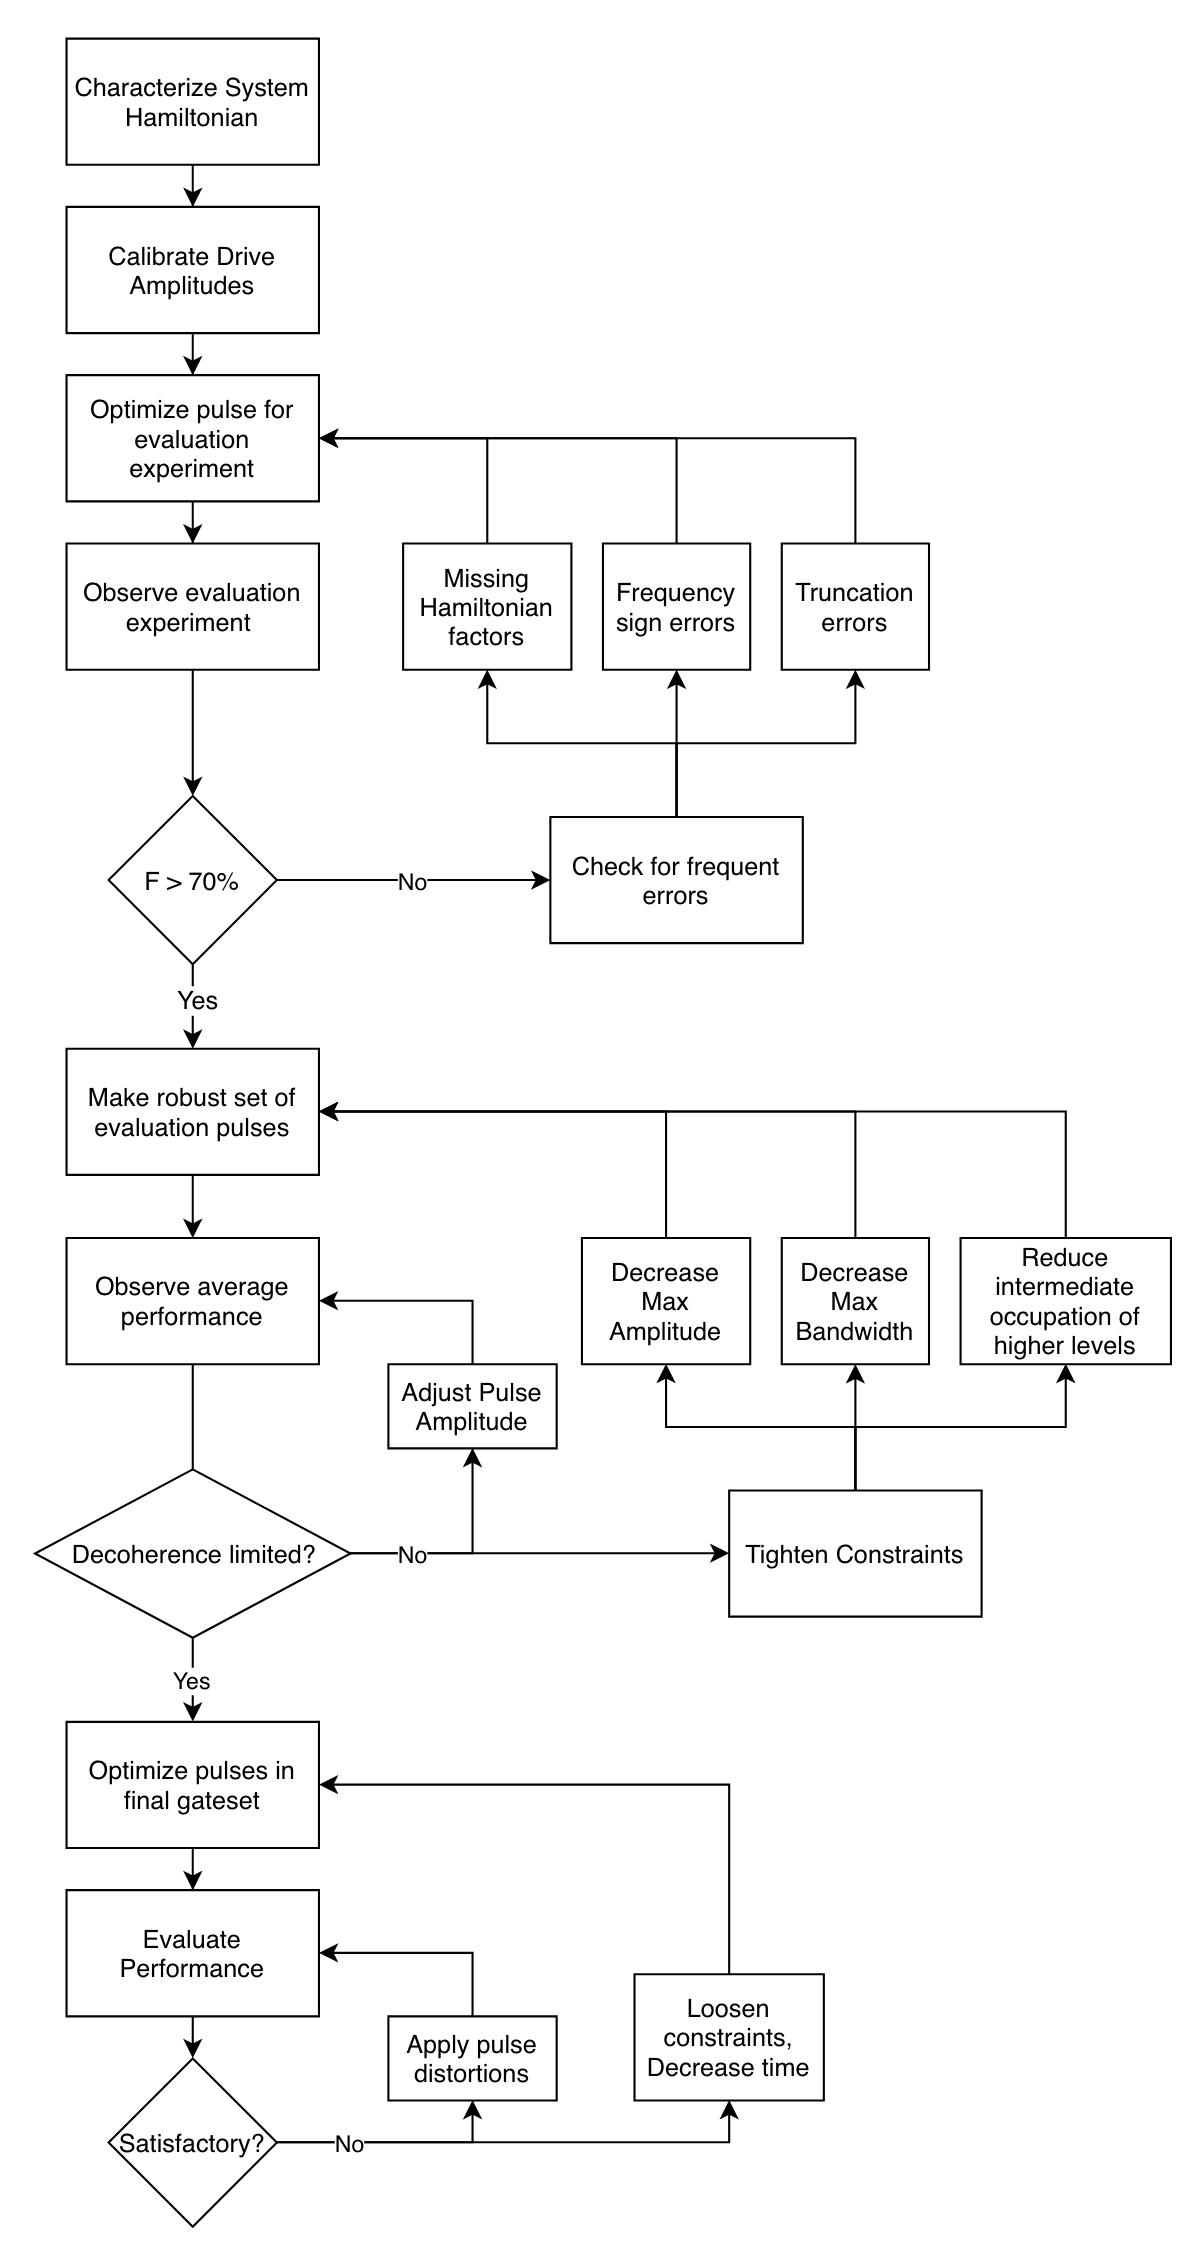
\includegraphics[width=0.6\linewidth]{flowchart.png}
    \caption{Flowchart for optimal control system}
    \label{fig:flowchart}
\end{figure}

%%%%%%%%%%%%%%%%%%%%%%%%%%%%%%%
\subsection{unselective spin flip, cavity coupled with single qubit(effective)}

%%%%%%%%%%%%%%%%%%%%%%%%%%%%%%%
\subsection{selective spin flip, cavity coupled with single qubit(effective)}

%%%%%%%%%%%%%%%%%%%%%%%%%%%%%%%
\subsection{vacuum to cat state, cavity coupled with single qubit(effective)}

%%%%%%%%%%%%%%%%%%%%%%%%%%%%%%%%%%%%%%%%%%%%%%%%%%%%%%%%%%%%%%%
\section{Physical realizability}
go back the Hamiltonian massagiing: Perturbation, frame change, throwing away small cross terms, exact \\
compare fidelity

\section{Future work}

\section{Conclusion}


\end{document}